\documentclass[11pt,a4paper]{article}

\usepackage[margin=2.2cm]{geometry}
\usepackage[T1]{fontenc}
\usepackage{graphicx}
\usepackage{float}
\usepackage{booktabs}
\usepackage{xcolor}
\usepackage{listings}
\usepackage{longtable}

\definecolor{codebg}{gray}{0.96}
\definecolor{codeframe}{gray}{0.75}
\definecolor{keyc}{RGB}{0,80,140}
\definecolor{strc}{RGB}{140,60,20}
\definecolor{comc}{gray}{0.42}

\lstdefinelanguage{json}{
  morestring=[b]",
  morekeywords={true,false,null},
  sensitive=true,
  comment=[l]{//},
}

\lstdefinestyle{json}{
  language=json,
  basicstyle=\ttfamily\scriptsize,
  backgroundcolor=\color{codebg},
  frame=single, rulecolor=\color{codeframe}, framesep=5pt,
  breaklines=true, breakatwhitespace=true,
  columns=fullflexible, keepspaces=true, showstringspaces=false,
  keywordstyle=\color{keyc}, stringstyle=\color{strc},
  commentstyle=\color{comc}\itshape,
  aboveskip=8pt, belowskip=8pt,
}

\lstdefinestyle{sql}{
  language=SQL,
  basicstyle=\ttfamily\scriptsize,
  backgroundcolor=\color{codebg},
  frame=single, rulecolor=\color{codeframe}, framesep=5pt,
  breaklines=true, columns=fullflexible, showstringspaces=false,
  keywordstyle=\color{keyc}, stringstyle=\color{strc},
  commentstyle=\color{comc}\itshape,
  aboveskip=8pt, belowskip=8pt,
}

\setlength{\parindent}{0pt}
\setlength{\parskip}{6pt}

\newcommand{\pk}[1]{\underline{#1}}
\newcommand{\fk}[1]{\textit{#1}$^{\dagger}$}

% Page-breakable, hanging-indent replacement for the old tabbing block.
\newcommand{\schemaline}[1]{%
  \par\hangindent=1.6em\hangafter=1 #1\par\vspace{3pt}%
}

\pagestyle{plain}

\begin{document}

\begin{center}
{\Large\bfseries TOETAE SPECIAL}\\[2mm]
{\large Schema overview and API}
\end{center}

\vspace{2mm}

\section{Schema}

\begingroup
\setlength{\parskip}{0pt}
\schemaline{\texttt{permission}(\pk{id}, can\_overwrite, can\_edit\_role)}
\schemaline{\texttt{role}(\pk{id}, name, description, \fk{permission\_id})}
\schemaline{\texttt{account}(\pk{id}, username, email, \fk{role\_id}, quota, active)}
\schemaline{\texttt{status}(\pk{id}, name)}
\schemaline{\texttt{category}(\pk{id}, name)}
\schemaline{\texttt{task}(\pk{id}, name, description, \fk{status\_id}, \fk{category\_id},
  \fk{created\_by}, \fk{completed\_by}, created, updated, completed\_at, due\_date)}
\schemaline{\texttt{task\_assigned\_to}(\pk{\fk{task\_id}}, \pk{\fk{assigned\_id}})}
\schemaline{\texttt{ticket}(\pk{id}, name, description, \fk{status\_id}, \fk{category\_id},
  \fk{created\_by}, \fk{completed\_by}, \fk{assigned\_id}, created, updated,
  completed\_at, due\_date)}
\schemaline{\texttt{announcement}(\pk{id}, name, description, \fk{status\_id},
  \fk{created\_by}, created, updated)}
\schemaline{\texttt{audit\_log}(\pk{id}, from\_table, row\_id, column\_name, old\_value,
  new\_value, \fk{by\_whom}, occurred\_at)}
\endgroup

{\footnotesize \pk{Underlined} = primary key. \fk{Italic} = foreign key.\par}

\begin{figure}[H]
\centering
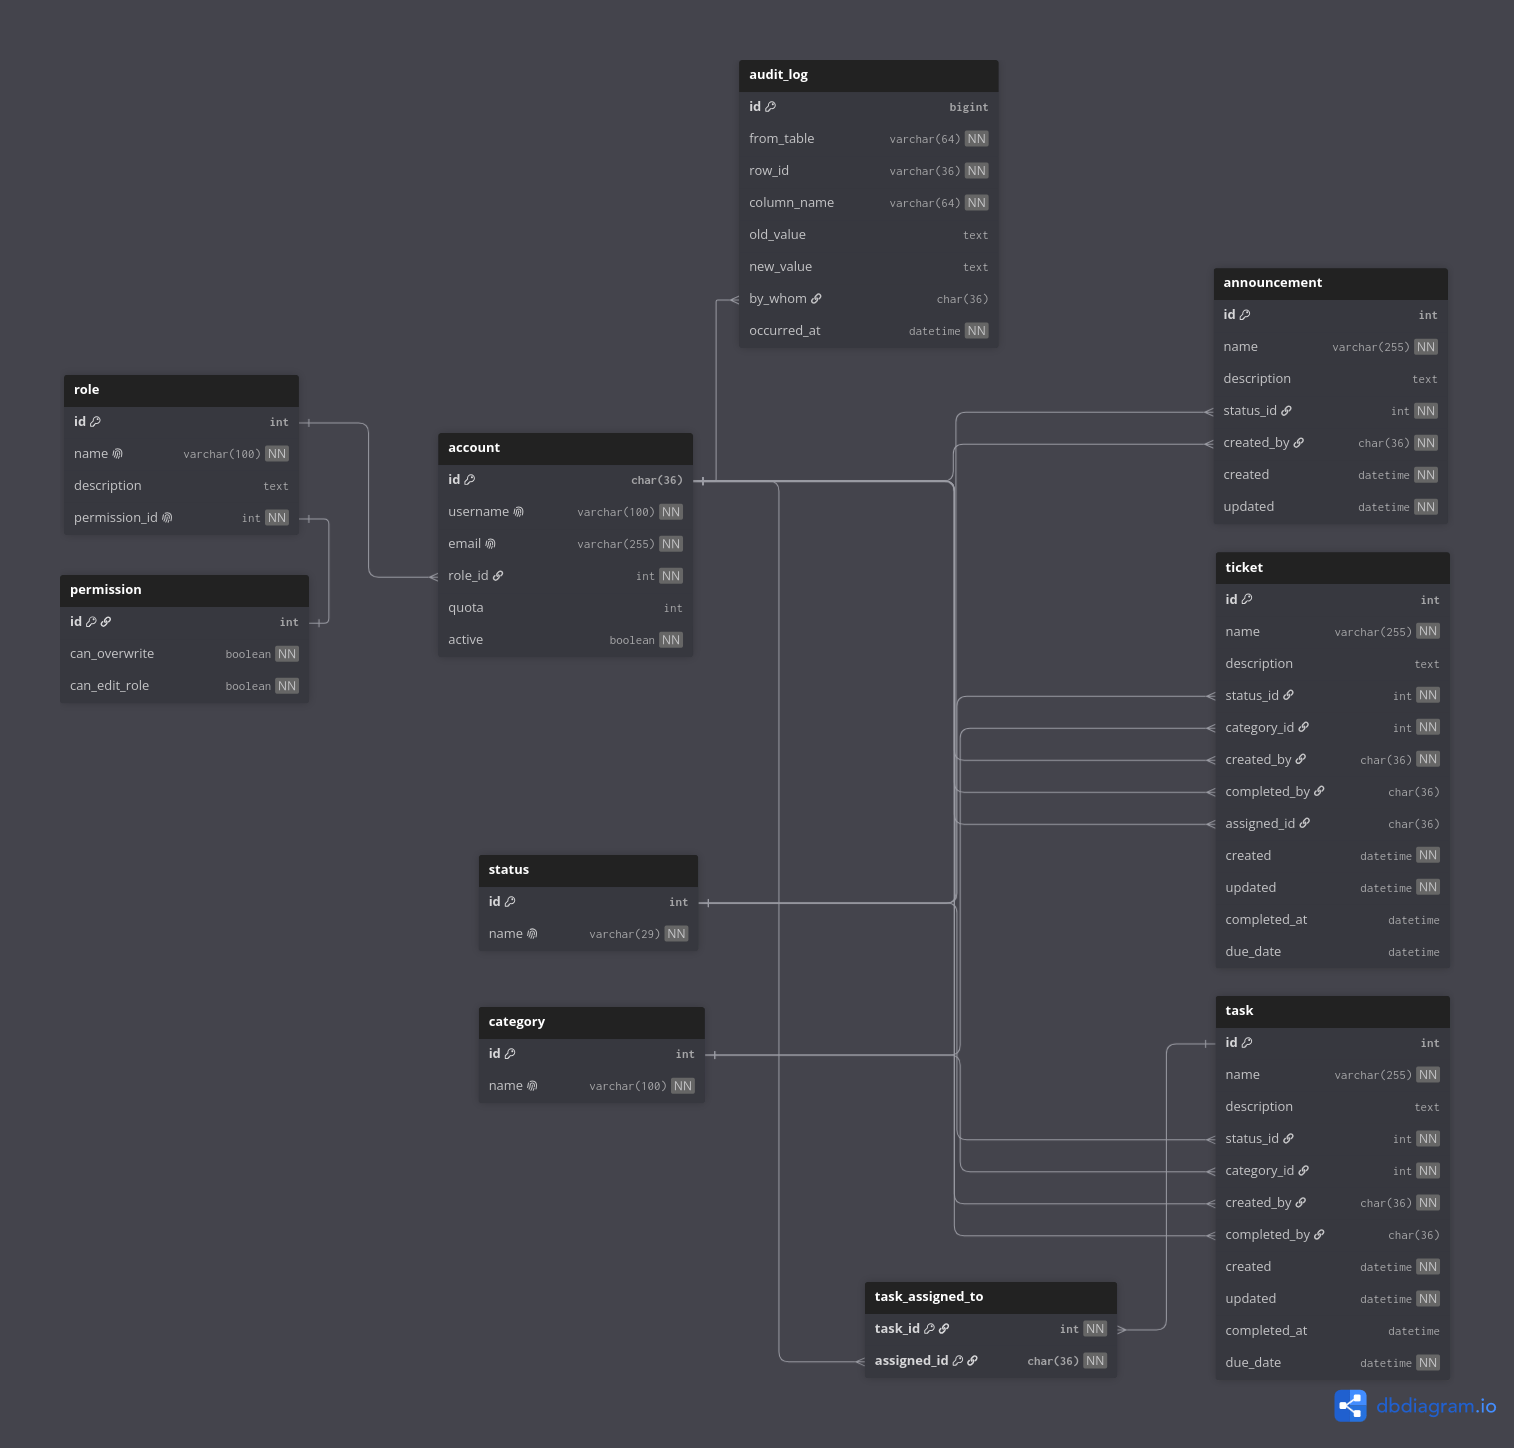
\includegraphics[width=\textwidth,height=12.4cm,keepaspectratio]{erd.png}
\end{figure}

\clearpage
\section{Before We Begin}

Before implementation begins, please read through the API
requirements below.

The purpose of this section is to establish a few common
agreements so that the backend and frontend can be implemented
without making conflicting assumptions.

\subsection{Roles}

\begin{longtable}{@{}p{4.0cm}p{12.18cm}@{}}
\toprule
\textbf{Role} & \textbf{Permissions} \\
\midrule
\endhead

Lab Admins &
Have access to create, edit, update, and delete every request
(tickets and tasks). They may also create user accounts and grant roles.
User accounts are never deleted. Instead, an account is
deactivated by setting \texttt{active} to \texttt{false}.
\\[6pt]

Lab Users & May create, edit, update, and delete only their own requests.
The exception is a task assigned to everyone. In that case,
any user may update the task's status.
\\

\bottomrule
\end{longtable}


\subsection{Status}

The \texttt{status} table is fixed.

The workflow always uses the same five status values, and
records reference them through \texttt{status\_id}.

The \texttt{status} query parameter described later accepts
only these five status names.

\begin{longtable}{@{}p{1.4cm}p{3.0cm}p{11.36cm}@{}}
\toprule
\textbf{ID} & \textbf{Name} & \textbf{Description} \\
\midrule
\endhead

1 & Pending &
Newly submitted and not yet reviewed.
\\

2 & Approve &
Reviewed and approved. Work has not necessarily started yet.
\\

3 & Reject &
Reviewed and declined. No further action is expected.
\\

4 & In-Progress &
Approved and currently being worked on.
\\

5 & Complete &
Finished.

Excluded from the dashboard view and visible only in the
request table.
\\

\bottomrule
\end{longtable}

Status ordering can simply follow \texttt{status.id}, which
naturally produces:

\begin{center}
\texttt{Pending}
$\rightarrow$
\texttt{Approve}
$\rightarrow$
\texttt{Reject}
$\rightarrow$
\texttt{In-Progress}
$\rightarrow$
\texttt{Complete}
\end{center}

\pagebreak
\subsection{Category}

Unlike \texttt{status}, the \texttt{category} table is
dynamic.

Lab staff may define their own categories. The following rows
are example seed data only and are \textbf{not} part of the
fixed specification.

\begin{longtable}{@{}p{1.4cm}p{4.4cm}p{9.96cm}@{}}
\toprule
\textbf{ID} & \textbf{Name} & \textbf{Description} \\
\midrule
\endhead

1 & Safety \& Compliance & Example only. \\
2 & Reagents \& Consumables & Example only. \\
3 & Sample Prep & Example only. \\
4 & Instrumentation & Example only. \\
5 & Data Analysis & Example only. \\

\bottomrule
\end{longtable}

Because categories are configurable, no endpoint should
hard-code a category name or assume that a particular
\texttt{category\_id} will always exist.


% ============================================================
\clearpage
\section{API Requirements}
% ============================================================

\begin{center}
\fbox{
\parbox{0.9\textwidth}{
\centering
\textbf{This is a guide, not a prison.}\\[2pt]
\footnotesize
The response structures shown below are suggested examples to
make frontend development easier.

The final implementation does not have to follow them
character-for-character. As long as the API remains
consistent, predictable, and documented, feel free to
structure the endpoints however you think is best.

}
}
\end{center}


\section{GET /tasks}

Retrieves tasks available to the current user.

% ------------------------------------------------------------
\subsection{Optional Query Parameters}
% ------------------------------------------------------------

\begin{longtable}{@{}p{3.0cm}p{13.18cm}@{}}
\toprule
\textbf{Parameter} & \textbf{Description} \\
\midrule
\endhead

\texttt{status} &
Filter tasks by status.

Only the five predefined status names are accepted.
\\

\texttt{category} &
Filter tasks by category name.
\\

\texttt{onlyDueDate} &
When \texttt{true}, return only tasks whose due date has not
passed.
\\

\bottomrule
\end{longtable}


% ------------------------------------------------------------
\subsection{Dashboard Behaviour}
% ------------------------------------------------------------

When \texttt{onlyDueDate=true} is supplied without any other
filters, the endpoint is intended to provide the tasks shown
on the dashboard.

For the dashboard, only tasks with status
\texttt{In-Progress} should be returned.

\begin{longtable}{@{}p{3.0cm}p{13.18cm}@{}}
\toprule
\textbf{Caller} & \textbf{Behaviour} \\
\midrule
\endhead

Admin &
Returns every task.

No ownership or assignment filter is applied.

Results are ordered by \texttt{status.id}.
\\[4pt]

Non-admin &
Returns only tasks assigned to the caller through
\texttt{task\_assigned\_to}.

Results are ordered by due date, followed by status.
\\

\bottomrule
\end{longtable}

The scope of a non-admin user's task list is determined by the
assignment table, \textbf{not} by \texttt{created\_by}.

Therefore, a user who created a task but was never assigned to
it does not automatically see the task on their dashboard.

\newpage
\subsection{Example Response}

\begin{lstlisting}[style=json]
{
  "Tasks": [
    {
      "name": "Validate autoclave cycle with spore strips",
      "description": "...",
      "status": "In-Progress",
      "category": "Safety & Compliance",
      "due_date": "2026-08-20T17:00:00",
      "created_by": "h.nakamura"
    },
    {
      "name": "Reconcile reagent inventory against orders",
      "description": "...",
      "status": "In-Progress",
      "category": "Reagents & Consumables",
      "due_date": "2026-09-02T17:00:00",
      "created_by": "h.nakamura"
    },
  ]
}
\end{lstlisting}

No task in the seed data is \texttt{Pending},
\texttt{Approve}, or \texttt{Reject}.

Therefore, the admin list contains six
\texttt{In-Progress} tasks followed by two
\texttt{Complete} tasks.

% ------------------------------------------------------------
\subsection{Example: Non-admin User}
% ------------------------------------------------------------

For user \texttt{h.nakamura}, four tasks are assigned to the

\begin{lstlisting}[style=json]
{
  "Tasks": [
    {
      "name": "Validate autoclave cycle with spore strips",
      "description": "...",
      "status": "In-Progress",
      "category": "Safety & Compliance",
      "due_date": "2026-08-20T17:00:00",
      "created_by": "h.nakamura"
    },
    {
      "name": "Re-run failed qPCR plate 14",
      "description": "...",
      "status": "In-Progress",
      "category": "Sample Prep",
      "due_date": "2026-09-19T17:00:00",
      "created_by": "h.nakamura"
    },
  ]
}
\end{lstlisting}


% ============================================================
\clearpage
\section{GET /tickets}
% ============================================================

Retrieves tickets available to the current user.

% ------------------------------------------------------------
\subsection{Optional Query Parameters}
% ------------------------------------------------------------

\begin{longtable}{@{}p{3.0cm}p{13.18cm}@{}}
\toprule
\textbf{Parameter} & \textbf{Description} \\
\midrule
\endhead

\texttt{status} &
Filter tickets by status.
\\

\texttt{category} &
Filter tickets by category.
\\

\texttt{onlyOwned} &
When \texttt{true}, return only tickets created by the caller.
\\

\bottomrule
\end{longtable}


% ------------------------------------------------------------
\subsection{Access Behaviour}
% ------------------------------------------------------------

\begin{longtable}{@{}p{3.0cm}p{13.18cm}@{}}
\toprule
\textbf{Caller} & \textbf{Behaviour} \\
\midrule
\endhead

Admin &
Returns every ticket.

No ownership filter is applied.

Results are ordered by \texttt{status.id}.
\\[4pt]

Non-admin &
Returns only tickets created by the caller:

\texttt{ticket.created\_by = :me}

Results are ordered by due date, followed by status.
\\

\bottomrule
\end{longtable}


% ------------------------------------------------------------
\subsection{Example: Admin}
% ------------------------------------------------------------

For example, an admin user such as
\texttt{e.vasquez} receives all seven tickets.

\begin{lstlisting}[style=json]
{
  "Tickets": [
    {
      "name": "Wrong lot of antibody shipped",
      "description": "...",
      "status": "Pending",
      "category": "Reagents & Consumables",
      "due_date": "2026-09-11T17:00:00",
      "created_by": "h.nakamura"
    },
    {
      "name": "Centrifuge vibrating at high speed",
      "description": "...",
      "status": "Pending",
      "category": "Instrumentation",
      "due_date": null,
      "created_by": "d.okonkwo"
    }
  ]
}
\end{lstlisting}

All five statuses appear in \texttt{status.id} order:

\begin{center}
Pending $\rightarrow$
Approve $\rightarrow$
Reject $\rightarrow$
In-Progress $\rightarrow$
Complete
\end{center}

\newpage
\subsection{Example: Non-admin User}

For user \texttt{h.nakamura}, three tickets were created by
the user.

\begin{lstlisting}[style=json]
{
  "Tickets": [
    {
      "name": "Freezer temperature log has gaps",
      "description": "...",
      "status": "Complete",
      "category": "Safety & Compliance",
      "due_date": "2026-07-29T17:00:00",
      "created_by": "h.nakamura"
    },
    {
      "name": "Request BSL-2 room access for new student",
      "description": "...",
      "status": "In-Progress",
      "category": "Safety & Compliance",
      "due_date": "2026-08-22T17:00:00",
      "created_by": "h.nakamura"
    },
    {
      "name": "Wrong lot of antibody shipped",
      "description": "...",
      "status": "Pending",
      "category": "Reagents & Consumables",
      "due_date": "2026-09-11T17:00:00",
      "created_by": "h.nakamura"
    }
  ]
}
\end{lstlisting}

Ticket 1 and Ticket 3 are both assigned to
\texttt{h.nakamura}, but they were created by
\texttt{d.okonkwo}.

Therefore, they do not appear in the non-admin result when
using the ownership rule above.

If the dashboard is intended to show all work a technician
needs to act on, the predicate can instead be:

\begin{lstlisting}[style=sql]
ticket.created_by = :me
OR ticket.assigned_id = :me
\end{lstlisting}


\clearpage
\section{POST / PUT / DELETE}

The exact implementation of the mutation endpoints is
intentionally left open.

Use whatever request and response structure makes the most
sense for the backend implementation, provided that the
following requirements are respected:

\begin{itemize}
    \item Authentication and authorization must be enforced.
    \item Admin users must be able to perform their permitted
          operations across all requests.
    \item Non-admin users must not modify requests they do not
          have permission to modify.
    \item User accounts must never be physically deleted.
          Deactivate them using \texttt{active=false}.
    \item Changes to important records should be compatible
          with the \texttt{audit\_log} table.
    \item Status and category references must remain valid.
    \item The API should return appropriate HTTP status codes.
    \item Request and response formats should remain
          consistent across endpoints.
\end{itemize}

\begin{center}
\fbox{
\parbox{0.82\textwidth}{
\centering
\textbf{POST? PUT? DELETE?}\\[3pt]
Do whatever makes the most sense.
Just don't break the database, authorization rules,
or whoever has to consume the API afterwards.
}
}
\end{center}


\section{General API Principles}

The following principles apply to all endpoints:

\begin{enumerate}
    \item The authenticated user determines the caller's
          permissions.

    \item Authorization must be enforced by the backend.
          The frontend must not be treated as a security
          boundary.

    \item Admin permissions are determined by the user's role
          and associated permissions.

    \item Non-admin access is restricted according to the
          ownership and assignment rules described above.

    \item Statuses are fixed and must not be dynamically
          created by normal request operations.

    \item Categories are dynamic and must be resolved through
          the \texttt{category} table.

    \item Dates should use a consistent ISO 8601-compatible
          representation on the database. For frontend just convert it to Thailand timezone.

    \item Deleted or deactivated resources should behave
          consistently across all endpoints.

    \item API behaviour should be documented whenever the
          implementation differs from the examples in this
          document.
\end{enumerate}


\section{Final Note}

The examples in this document are intended to communicate
\textbf{behaviour}, not to dictate every implementation detail.

If the backend implementation requires a different response
shape, additional fields, different mutation
routes, or other improvements, that is completely fine.

\begin{center}
\Large
\textbf{Build it however you want.}\\[2mm]
\normalsize
Just don't leak the API keys
\end{center}

\end{document}
